\documentclass[a4paper,10pt]{article}
\usepackage[utf8]{inputenc}
\usepackage{tikz}
\usepackage{amsmath}
\usepackage{fullpage}

%opening
\title{Attaque du protocole de l'équipe Brachistochrone}
\author{par l'Equipe Stone Jaws}
\date{4 octobre 2018}

\begin{document}

\maketitle

\section{Le protocole}

Considérons 3 rôles $i$, $r$, et $m$ (que l'on appellera respectivement initiateur, récepteur, et serveur). Dans la suite, on considèrera $\textrm{getNonce}$ comme une constante publique. La sémantique (en utilisant les notations de \cite{cas}) de ce protocole est alors donnée par :
\begin{eqnarray*}
	TdSD(i) & = & \{ (i,r,m, K, K_{im}, \textrm{getNonce}), \\
		& & \texttt{send}_1(i,m, \textrm{getNonce} ), \\
		& & \texttt{recv}_2(m,i,  \textrm{senc}(V,K_{im}) ),\\
		& & \texttt{send}_3(i,m, \langle \textrm{senc}(h(V),K_{im}),  \textrm{senc}(\langle r, K \rangle,K_{im})\rangle   )  \\
		& & \texttt{recv}_7(r,i, h(K) ) \} \\
\end{eqnarray*}
\begin{eqnarray*}
	TdSD(r) & = & \{ (i,r,m, K_{rm}, \textrm{getNonce}, N_b), \\
		& & \texttt{recv}_4(m,r, \textrm{getNonce} ), \\
		& & \texttt{send}_5(r,m,  \textrm{senc}(N_b,K_{rm}) ),\\
		& & \texttt{recv}_6(m,r, \langle \textrm{senc}(h(N_b),K_{rm}),  \textrm{senc}(\langle i, W \rangle,K_{im})\rangle  ) \\
		& & \texttt{send}_7(r,i, h(W)  ) \} \\
\end{eqnarray*}
\begin{eqnarray*}
	TdSD(m) & = & \{ (i,r,m, K_{rm}, K_{im}, getNonce, N_s), \\
		& & \texttt{recv}_1(i,m, \textrm{getNonce} ), \\
		& & \texttt{send}_2(m,i, \textrm{senc}(N_s,K_{im})  ) \\
		& & \texttt{recv}_3(i,m, \langle \textrm{senc}(h(N_s),K_{im}),  \textrm{senc}(\langle r, U \rangle,K_{im})\rangle   ) \\
		& & \texttt{send}_4(m,r, \textrm{getNonce} ), \\
		& & \texttt{recv}_5(r,m, \textrm{senc}(X,K_{rm})  ) \\
		& & \texttt{send}_6(m,r, \langle \textrm{senc}(h(X),K_{rm}),  \textrm{senc}(\langle r, U \rangle,K_{rm})\rangle   ) \} \\
\end{eqnarray*}


\begin{center}

\begin{figure}
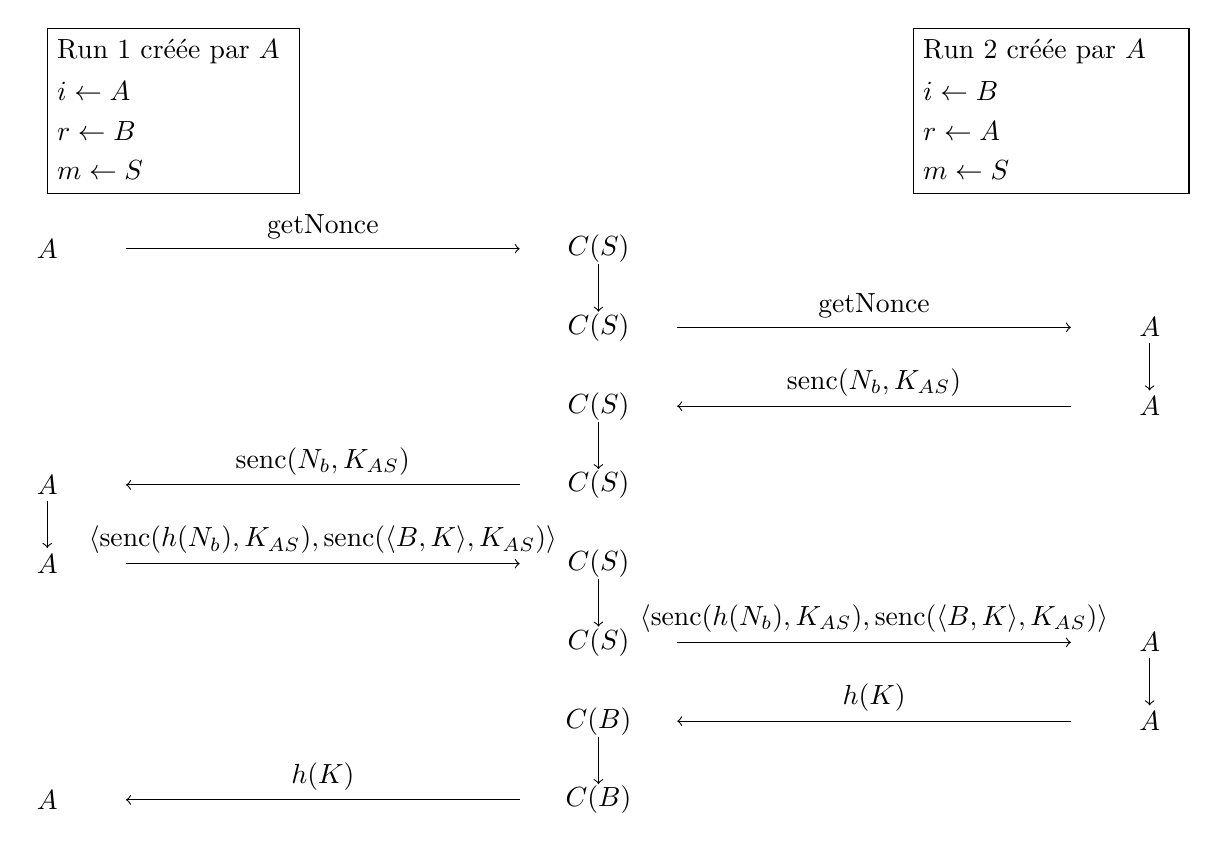
\begin{tikzpicture}
        \draw(-7,8.8) rectangle (-3.8,6.7);
	\draw (-7,8.5) node[right]{Run 1 créée par $A$};
	\draw (-7,8) node[right]{$i \leftarrow A$};
	\draw (-7,7.5) node[right]{$r \leftarrow B$};
	\draw (-7,7) node[right]{$m \leftarrow S$};
	\draw(4,8.8) rectangle (7.5,6.7);
	\draw (4,8.5) node[right]{Run 2 créée par $A$};
	\draw (4,8) node[right]{$i \leftarrow B$};
	\draw (4,7.5) node[right]{$r \leftarrow A$};
	\draw (4,7) node[right]{$m \leftarrow S$};
	\draw (-7,6) node{$A$} ;
	\draw[->]  (-6,6) -- node[above]{$\textrm{getNonce}$} (-1,6);
	\draw (0,6) node{$C(S)$} ;
	\draw[->]  (0,5.8) -- (0,5.2) ;
	\draw (0,5) node{$C(S)$} ;
	\draw[->]  (1,5) -- node[above]{$\textrm{getNonce}$} (6,5) ;
	\draw (7,5) node{$A$} ;
	\draw[->]  (7,4.8) -- (7,4.2) ;
	\draw (7,4) node{$A$} ;
	\draw[->]  (6,4) -- node[above]{$\textrm{senc}(N_b,K_{AS})$} (1,4) ;
	\draw (0,4) node{$C(S)$} ;
	\draw[->]  (0,3.8) -- (0,3.2) ;
	\draw (0,3) node{$C(S)$} ;
	\draw[->]  (-1,3) -- node[above]{$\textrm{senc}(N_b,K_{AS})$} (-6,3) ;
	\draw (-7,3) node{$A$} ;
	\draw[->]  (-7,2.8) -- (-7,2.2) ;
	\draw (-7,2) node{$A$} ;
	\draw[->]  (-6,2) -- node[above]{$ \langle \textrm{senc}(h(N_b),K_{AS}),  \textrm{senc}(\langle B, K \rangle,K_{AS})\rangle $} (-1,2) ;
	\draw (0,2) node{$C(S)$};
	\draw[->]  (0,1.8) -- (0,1.2) ;
	\draw (0,1) node{$C(S)$} ;
	\draw[->]  (1,1) -- node[above]{$\langle \textrm{senc}(h(N_b),K_{AS}),  \textrm{senc}(\langle B, K \rangle,K_{AS})\rangle$} (6,1) ;
	\draw (7,1) node{$A$};
	\draw[->] (7,0.8) -- (7,0.2) ;
	\draw (7,0) node{$A$};
	\draw[->] (6,0) -- node[above]{$h(K)$} (1,0) ;
	\draw (0,0) node{$C(B)$};
	\draw[->] (0,-0.2) -- (0,-0.8);
	\draw (0,-1) node{$C(B)$};
	\draw[->] (-1,-1) -- node[above]{$h(K)$} (-6,-1) ;
	\draw (-7,-1) node{$A$};
\end{tikzpicture}
\caption{Attaque du protocole Brachistochrone}
\label{fig1}
\end{figure}
\end{center}



\section{Attaque sur le protocole}
L'attaque est représentée sur la Figure \ref{fig1} et fonctionne comme suit : $A$ exécute le protocole une fois (dans la Run $1$) en tant qu'initiateur et veut s'adresser à $B$, et une autre fois (dans la Run $2$) en tant que récepteur avec $B$ dans le rôle d'initiateur. On notera $A_1$ et $A_2$ pour distinguer l'agent $A$ en tant qu'acteur des Runs $1$ et $2$.\\
\begin{enumerate}
\item $A_1$ envoie un premier message $\textrm{getNonce}$ au serveur, qui est intercepté par un agent malveillant $C$. Celui redirige exactement ce message à $A_2$, qui croit que $B$ désire communiquer avec lui par l'intermédiaire du serveur.
\item $A_2$ envoie alors à $S$ le nonce encrypté $\textrm{senc}(N_b,K_{AS})$, qui est intercepté par $C$. Ce dernier le redirige vers $A_1$.
\item $A_1$ pense alors que $S$ lui a envoyé le nonce qu'il a prélablement demandé, et répond au challenge, puis donne son message et le destinaire, sous la forme $\langle \textrm{senc}(h(N_b),K_{AS}),  \textrm{senc}(\langle B, K \rangle,K_{AS})\rangle$. Ce message est intercepté par $C$ et redirigé vers $A_2$. Celui-ci croit alors que $S$ a répondu a son challenge et que $B$ lui transmet le message $K$.
\item $A_2$ accuse alors réception à $B$ du message $K$ en envoyant $h(K)$, $C$ intercepte le message et le redirige vers $A_1$, qui croit que $B$ accuse réception du message $K$ que $A_1$ lui avait envoyé.
\end{enumerate}

On remarque alors que deux des propriétés exigées ne sont pas vérifiées :
\begin{itemize}
\item Dans cet exemple, l'initiateur de la Run $1$ envoie un message à un récepteur et termine le protocole alors que le récepteur n'a pas reçu le message. 
\item De plus, le récepteur de la Run $2$ peut croire recevoir une donnée d'un initiateur qui ne l'a en fait jamais envoyée.
\end{itemize}

\bibliographystyle{plain}
\bibliography{ref.bib}

\end{document}
